\begin{tikzpicture}[font=\sffamily,>=triangle 45]
 \def\radius{1.mm} 
  % place dffs and draw connections

  \renewcommand{\dname}{$D$}
\renewcommand{\qname}{$Q$}
\newcommand{\qbarname}{$\overline{Q}$}
\newcommand{\clkname}{}
\input{flipflop.tex}
  \node [shape=dff] (DFF0) at (0,0) {};

  \node [shape=dff] (DFF1) at (0,3) {};

   \node [shape=dff] (DFF2) at (0,6) {};


 
  \node[nor gate US, draw, logic gate inputs=nn, anchor=input 1] at
 ($(DFF1.D)-(1.5,-0.1)$) (nor0) {};
 \node[and gate US, draw, logic gate inputs=nn, anchor=input 1] at
 ($(DFF0.D)-(1.5,-0.1)$) (and0) {};
 \draw[-,name path = line 3] (DFF2.Q) --(2,6.4) -- (2,7.5) -- (-3,7.5) -- (-3,3.4)  |- (nor0.input 2);
 
  \path[name path = line 1] (DFF0.Q) --(2.5,.4);
  \draw[-]  (2.5,0.4) --(2.5,7.2);
  \path[name path = line 4] (2.5,7.2) -- (-2.5,7.2);
  \draw (-2.5,7.2)-- (-2.5,3.8)  |- (nor0.input 1);
  
   \draw[name path = line 2] (DFF1.Q) --(1.7,3.4) -- (1.7,-1.5) -- (-2.5,-1.5) -- (-2.5,0.4)  |- (and0.input 1);
   \draw[-] (DFF0.Qn) --(1,-.4) -- (1,-1) -- (-2.2,-1) -- (-2.2,0.3)  |- (and0.input 2);
  
   \draw (-2.5,6.4) -- (DFF2.D);
   \node[above] at (1,6.4){P};
   \node[above] at (1,3.4){Q};
   \node[above] at (1,.4){R};
   \draw[-] (-0.6,-0.4) -- (-1,-.4);
   \draw[-] (-0.6,2.6) -- (-1,2.6);
   \draw[-] (-0.6,5.6) -- (-1,5.6);
   \node[above] at (-1.5,5.4) {Clock};
   \node[above] at  (-1.5,2.4) {Clock};
   \node[above] at (-1.5,-.6) {Clock};
   

%%%%%%%%%%%%%%%%%%
  
   \path [name intersections={of = line 1 and line 2}];
  \coordinate (S)  at (intersection-1);
   % path a circle around this intersection for the arc
  \path[name path=circle] (S) circle(\radius);
   % find intersections of second line and circle
  \path [name intersections={of = circle and line 1}];
  \coordinate (I1)  at (intersection-1);
  \coordinate (I2)  at (intersection-2);
  
 %\tkzDrawArc[color=black](S,I1)(I2);
   \draw[-] (DFF0.Q) -- (1.6,0.4);
  \draw[-] (1.8,0.4) -- (2.5,0.4);
  
  %%%%%%%%%%%%%%%%%%
\path [name intersections={of = line 3 and line 4}];
 \coordinate (S1)  at (intersection-1);
  % path a circle around this intersection for the arc
  \path[name path=circle] (S1) circle(\radius);
   % find intersections of second line and circle
  \path [name intersections={of = circle and line 4}];
  \coordinate (I3)  at (intersection-1);
  \coordinate (I4)  at (intersection-2);
  
 \tkzDrawArc[color=black](S1,I4)(I3);
   \draw[-] (-2.5,7.2) -- (1.9,7.2);
  \draw[-] (2.1,7.2) -- (2.5,7.2);
 
  %%%%%%%%%%%
  
\draw[-] (nor0.output) -- (DFF1.D);
\draw[-] (and0.output) -- (DFF0.D);

\end{tikzpicture}

%https://gateoverflow.in/216667/isi-2018-mma-2?show=216701#a216701
\documentclass[tikz]{standalone}
\usepackage{pgfplots}
\pgfplotsset{compat=1.11}
\usepgfplotslibrary{fillbetween}
\usetikzlibrary{intersections}
\usepackage{tkz-euclide}
\begin{document}
\begin{figure}[h]
\begin{tikzpicture}
   \tkzInit[xmax=6,ymax=6,xmin=-6,ymin=-6]
   \tkzGrid
   \tkzAxeXY
   \draw[name path = A, thick,latex-latex] (-1,2) -- (2,-1) node[anchor=south west] {}; % two points for drawing x+y=1
   
    \draw[ name path = B,thick,latex-latex] (1,2) -- (-2,-1) node[anchor=south east] {}; % two points for drawing x+y=2
    
     \filldraw[ name path = C,thick,latex-latex] (-2,1) -- (1,-2) node[anchor=south west] {}; % two points for drawing 2x+y=2
      \filldraw[ name path = D,thick,latex-latex] (2,1) -- (-1,-2) node[anchor=south east] {}; % two points for drawing 2x+y=2
    \draw
            (-1,0)  -- (0, 1) -- (1,0) -- (0,-1) -- (-1,0);
            \fill[pattern=north west lines]
              (-1,0)  -- (0, 1) -- (1,0) -- (0,-1) -- (-1,0);

  \tkzText[above](0,7.75){Figure A}
    \tkzText[above](0,6.75){region covered by the graph $|X|+|Y| < = 1$}
  \tkzText[above,fill= orange!50](2,0.5){x + y = 1}
  
  \tkzText[above,fill= orange!50](-2,0.5){-x + y = 1}
  
  \tkzText[above,fill= orange!50](2,-1.5){-x - y = 1}
  
  \tkzText[above,fill= orange!50](-2,-1.5){x - y = 1}
  



  \end{tikzpicture}
  
  
  

\end{figure}

\end{document}
%%%https://gateoverflow.in/2608/gate1995-1-21?show=29554#a29554
\documentclass[border=4mm]{standalone}
\usepackage{pgfplots}
\pgfplotsset{compat=1.12}
\begin{document}
  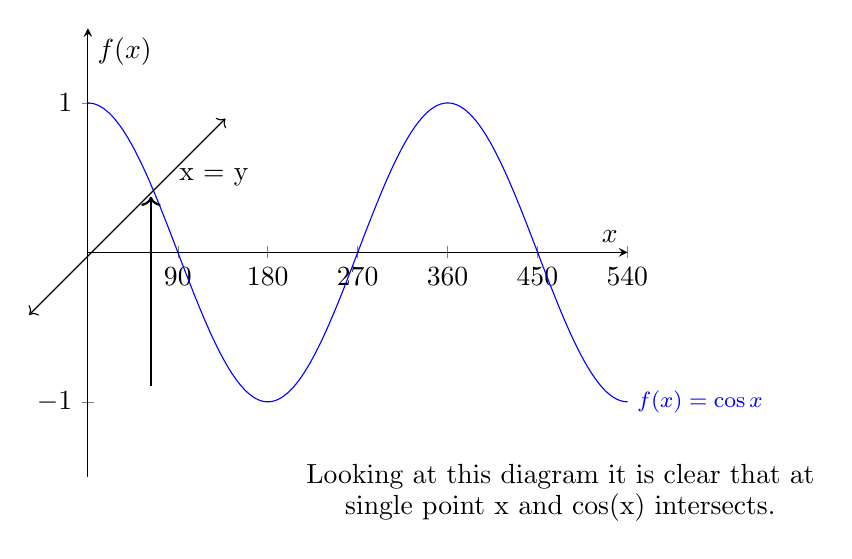
\begin{tikzpicture}
    \begin{axis}[
     clip=false,
     xmin=0,xmax=3*pi,
     xlabel= $x$,
     ylabel=$f(x)$,
     ymin=-1.5,ymax=1.5,
     axis lines=middle,
     %axis x line=middle,
     %axis y line=left,
%     axis x line=middle,
     xtick={0,1.57,3.14,4.71,6.28,7.85,9.42},
     xticklabels={$0$,$90$,$180$,$270$,$360$,$450$,$540$},
     %xticklabel style={anchor=north west}
     ]
     
      \addplot[domain=0:3*pi,samples=200,blue]{cos(deg(x))}
        node[right,pos=1,font=\footnotesize]{$f(x)=\cos x$};
    \end{axis}
  
        \draw[<->,shorten >=-3em,shorten <=-3em] (0,2.8) -- (1,3.8);
         \draw[<-,shorten >=-3em,shorten <=-3em,thick] (0.8,2.5) -- (.8,2.2);
    \node at (6,0){Looking at this diagram it is clear that at};
        \node at (6,-0.4){single point x and cos(x) intersects.};
        \node at (1.6,3.8){x = y};
  \end{tikzpicture}
\end{document}


%%%%%%%%%%https://gateoverflow.in/118292/gate2017-1-12?show=120564#a120564
documentclass[border=4mm]{standalone}
\usepackage{tikz}
\usetikzlibrary{shapes,positioning,arrows,calc}

\begin{document}

\begin{tikzpicture}[stack/.style={
  rectangle split, rectangle split parts=5, draw, anchor=center},
  myarrow/.style={single arrow, draw=none}]



\node [draw,rectangle,align=left,right=of ini,label=above:{}] (mid)
  {Static Single assignment\\ $\dot$ Each assignment to a temporary is given a unique name\\$\dot$All of the uses reached by that assignment are renamed};

\node[font= \huge] at (2.5,-2) {p = a - b};
 
\node[font= \huge] at (2.5,-3) {q = p * c};
\node[font= \huge] at (2.5,-4) {p = u * v};
\node[font= \huge] at (2.5,-5) {q = p + q};
\draw[-,color= cyan] (1,-2) -- (0.5,-2) -- (0.5,-4) -- (1,-4);

\draw[-,color= cyan] (1,-3) -- (0,-3) -- (0,-5) -- (1,-5);
\draw[-,color= cyan] (5.3,-1)--(5.3,-6);
\node[font= \huge] at (8,-2) { = a - b};
\node[circle, inner sep=0pt, minimum size=1cm, color=white, fill=cyan] at (6.3,-2){$p_1$};
\node[circle, inner sep=0pt, minimum size=1cm, color=white, fill=cyan] at (8,-3){$p_1$};
\node[circle, inner sep=0pt, minimum size=1cm, color=white, fill=cyan] at (6.3,-3){$q_1$};
\node[circle, inner sep=0pt, minimum size=1cm, color=white, fill=cyan] at (6.3,-4){$p_2$};
\node[circle, inner sep=0pt, minimum size=1cm, color=white, fill=cyan] at (8,-5){$p_2$};
\node[circle, inner sep=0pt, minimum size=1cm, color=white, fill=cyan] at (9.6,-5){$q_1$};
\node[font= \huge] at (7.1,-3) {=};
\node[font= \huge] at (8,-4) { = u * v};
\node[font= \huge] at (7.1,-5) {= };
\node[font= \huge] at (8.7,-5) {+};
\node[font= \huge] at (9.1,-3) {* c};
\node[font= \huge] at (6.3,-5) {$q_2$};
\draw[->](6.6,-2)--(7.5,-2.7);
\draw[->](6.3,-3)--(9,-4.6);
\draw[->](6.6,-4)--(7.5,-4.6);

\end{tikzpicture}

\end{document}


%%%%%%%%%%%%%%
%https://gateoverflow.in/18392/tifr2010-a-13?show=18401#a18401

\documentclass[border=40mm]{standalone}


\usepackage{tikz}
\usetikzlibrary{calc,patterns}
\usepackage{rubikcube,rubikrotation,rubikpatterns}
\begin{document}

\begin{tikzpicture}
 \ShowCube{3.5cm}{0.7}{\DrawNCubeAll{10}{R}{G}{Y}}
 \draw[-,line width=0.3mm,pattern = north east lines] (-2.6,-4) --(-2.6,1.4) -- (2.6,1.4) -- (2.6,-4) -- cycle;
 
  \draw[-,line width=0.3mm,color= green] (3.1,1.4) -- (3.8,1.4) -- (3.8,-4)-- (3.1,-4) -- cycle;
  \node[draw,circle,color= white,line width=0.4mm ] at (3.4,2.2){};
  \draw[->,font=\huge,color=green,line width=0.5mm] (3.1,-2) -- (6.7,-2) node[right]{Two face colored};
   \draw[->,font=\huge,color=red,line width= 0.5mm] (0,1.4) -- (0,6.1) node[above]{one face colored};
    \draw[->,font=\huge,color=gray,line width=0.5mm] (3.4,2.2) -- (8,6) node[above]{Three face colored};
 
 \end{tikzpicture}

\end{document} 


%https://gateoverflow.in/27308/tifr2014-b-11?show=236529#a236529
% first image
\documentclass[margin=10pt]{standalone} 
\usepackage{tikz}
\usepackage{tikz-qtree}
\usetikzlibrary{trees,calc,arrows.meta,positioning,decorations.pathreplacing,bending}

\tikzset{
    edge from parent/.style={draw, thick, blue!70!black},
    no edge from this parent/.style={
        every child/.append style={
        edge from parent/.style={draw=none}}},
    level 3/.style={yshift=5cm},
    level 4/.style={level distance=5mm} 
         }

\begin{document}

\begin{tikzpicture}[
    level/.style={sibling distance=40mm/#1},
    text=blue!70!black,
    >=latex,
    font=\sffamily
    ]

\node (z){n} 
  child {node (a) {n/3}
    child {node  (b) {n/9}
      child {node (b1) {}[no edge from this parent]
       child {node (b11) {}}
      }
      child {node (b2) {}[no edge from this parent]
       child {node (b12) {}}
      }
    }
    child {node (g) {(3/12)n}
      child {node (g1) {}[no edge from this parent]
       child {node (g11) {}}
      }
      child {node (g2) {}[no edge from this parent]
       child {node (g12) {}}
      }
    }
  }
    child {node (d) {(3/4)n}
      child {node  (e) {(3/12)n}
        child {node (e1) {}[no edge from this parent]
         child {node (e11) {}}
        }
        child {node (e2) {}[no edge from this parent]
         child {node (e12) {}}
        }
      }
      child {node (f) {(9/16)n}
        child {node (f1) {}[no edge from this parent]
         child {node (f11) {}}
        }
        child {node (f2) {}[no edge from this parent]
         child {node (f12) {}
         }
         }
  }
};

\node[right=7 of z]  (ln1) {level 1}[no edge from this parent]
    child {node (ln2) {level 2}[no edge from this parent]
        child {node (ln3) {level 3}[no edge from this parent]
            child {node (ln4) {}[no edge from this parent]}}};
            
\draw[blue!70!black,thick,->]    
    ($(z.east)+(1em,0)$) -- (ln1);
\draw[blue!70!black,thick,->]    
    ($(a.east)+(13em,0)$) -- (ln2);
\draw[blue!70!black,thick,->]    
    ($(b.east)+(19em,0)$) -- (ln3);

\end{tikzpicture}

\end{document}

% second image 
\documentclass[margin=10pt]{standalone} 
\usepackage{tikz}
\usepackage{tikz-qtree}
\usetikzlibrary{trees,calc,arrows.meta,positioning,decorations.pathreplacing,bending}

\tikzset{
    edge from parent/.style={draw, thick, blue!70!black},
    no edge from this parent/.style={
        every child/.append style={
        edge from parent/.style={draw=none}}},
    level 3/.style={yshift=5cm},
    level 4/.style={level distance=5mm} 
         }

\begin{document}

\begin{tikzpicture}[
    level/.style={sibling distance=40mm/#1},
    text=blue!70!black,
    >=latex,
    font=\sffamily
    ]

\node (z){n} 
  child {node (a) {n/5}
    child {node  (b) {n/25}
      child {node (b1) {}[no edge from this parent]
       child {node (b11) {}}
      }
      child {node (b2) {}[no edge from this parent]
       child {node (b12) {}}
      }
    }
    child {node (g) {(3/20)n}
      child {node (g1) {}[no edge from this parent]
       child {node (g11) {}}
      }
      child {node (g2) {}[no edge from this parent]
       child {node (g12) {}}
      }
    }
  }
    child {node (d) {(3/4)n}
      child {node  (e) {(3/20)n}
        child {node (e1) {}[no edge from this parent]
         child {node (e11) {}}
        }
        child {node (e2) {}[no edge from this parent]
         child {node (e12) {}}
        }
      }
      child {node (f) {(9/16)n}
        child {node (f1) {}[no edge from this parent]
         child {node (f11) {}}
        }
        child {node (f2) {}[no edge from this parent]
         child {node (f12) {}
         }
         }
  }
};

\node[right=7 of z]  (ln1) {level 1}[no edge from this parent]
    child {node (ln2) {level 2}[no edge from this parent]
        child {node (ln3) {level 3}[no edge from this parent]
            child {node (ln4) {}[no edge from this parent]}}};
            
\draw[blue!70!black,thick,->]    
    ($(z.east)+(1em,0)$) -- (ln1);
\draw[blue!70!black,thick,->]    
    ($(a.east)+(13em,0)$) -- (ln2);
\draw[blue!70!black,thick,->]    
    ($(b.east)+(19em,0)$) -- (ln3);

\end{tikzpicture}

\end{document}



%https://gateoverflow.in/3757/gate2005-it-12?show=82151#a82151
\documentclass[tikz,border= 3mm]{standalone}
\usepackage{tikz-qtree}
\usetikzlibrary{positioning, shapes.geometric}
\smallskip
\begin{document}

% first diagram

\begin{tikzpicture}[level distance = 60pt, sibling distance = 30pt,
  edge from parent/.style = {
    draw, edge from parent path = {(\tikzparentnode) -- (\tikzchildnode.north)}},scale = 0.5]
  \tikzset{every internal node/.style = {draw, circle, font = \Large}}
  \tikzset{every leaf node/.style = {draw, regular polygon, regular polygon sides = 3, inner sep = 10pt}}

  
   \Tree[.$\times$
         ${}$
         ${}$
      ]
\node[below] at (-1.5,-2.8) {LST};
\node[below] at (1.5,-2.8) {RST}; 

\end{tikzpicture}

% second diagram
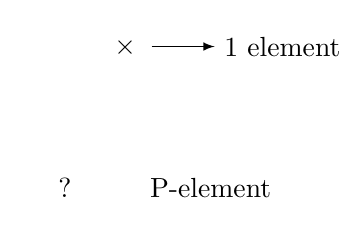
\begin{tikzpicture}[level distance = 70pt, sibling distance = 40pt,
  edge from parent/.style = {
    draw, edge from parent path = {(\tikzparentnode) -- (\tikzchildnode.north)}},scale = 0.5]
  \tikzset{every internal node/.style = {draw, circle, font = \Large}}
  \tikzset{every leaf node/.style = {draw, regular polygon, regular polygon sides = 3, inner sep = 10pt}}

   \Tree[.$\times$
         ${}$
         ${}$
      ]
\node[below] at (-1.8,-2.9) {?};
\node[below] at (1.9,-2.9) {P-element}; 
\node[right] at (2,0.2) {1 element};
\draw [->,>=latex] (0.4,0.2) -- (2,0.2);
\end{tikzpicture}

\end{document}








%%%%%%%%%%https://gateoverflow.in/2316/gate1993-19
\begin{tikzpicture}[font=\sffamily,>=triangle 45]
 \def\radius{1.mm} 
  % place dffs and draw connections

  \renewcommand{\dname}{}
\renewcommand{\qname}{}
\newcommand{\qbarname}{}
\newcommand{\clkname}{}
\input{flipflop.tex}
  \node [shape=dff] (DFF0) at (0,-0.1) {};

  \node [shape=dff] (DFF1) at (0,3.9) {};
\node[] at (-0.25,0.4){$D_B$};
\node[] at (0.35,0.4){$B$};
\node[] at (0.35,-0.4){$\overline{B}$};
\node[] at (-0.25,4.4){$D_A$};
\node[] at (0.35,4.4){$A$};
\node[] at (0.35,3.6){$\overline{A}$};
  


 
 \node[nand gate US, draw, logic gate inputs=nn, anchor=input 1] at
($(DFF0.D)-(2.2,-0.1)$) (nand1) {};

 \node[nand gate US, draw, logic gate inputs=nn, anchor=input 1] at
($(DFF1.D)-(2.2,-0.1)$) (nand2) {};


 \node[nand gate US, draw, logic gate inputs=nn, anchor=input 1] at
($(nand1.input 1)-(3.2,1.2)$) (nand3) {};


 \node[nand gate US, draw, logic gate inputs=nn, anchor=input 1] at
($(nand1.input 2)-(3.2,-1.2)$) (nand4) {};

 \node[nand gate US, draw, logic gate inputs=nn, anchor=input 1] at
($(nand2.input 1)-(3.2,1.2)$) (nand5) {};


 \node[nand gate US, draw, logic gate inputs=nn, anchor=input 1] at
($(nand2.input 2)-(3.2,-1.2)$) (nand6) {};
\draw[-] (nand1.output) -- (DFF0.D);
\draw[-] (nand2.output) -- (DFF1.D);

%\draw[-] (nand3.output) -- (-3.2,-1)  -- (-3.2,.3) --(nand1.input 2);



\end{tikzpicture}
